%%%%%%%%%%%%%%%%%%%%%%%%%%%%%%%%%%%%%%%%%%%%%%%%%%%%%%%%%%%%%%%%%%%%%%
% Overleaf (WriteLaTeX) Example: Molecular Chemistry Presentation
%
% Source: http://www.overleaf.com
%
% In these slides we show how Overleaf can be used with standard
% chemistry packages to easily create professional presentations.
%
% Feel free to distribute this example, but please keep the referral
% to overleaf.com
%
%%%%%%%%%%%%%%%%%%%%%%%%%%%%%%%%%%%%%%%%%%%%%%%%%%%%%%%%%%%%%%%%%%%%%%
% How to use Overleaf:
%
% You edit the source code here on the left, and the preview on the
% right shows you the result within a few seconds.
%
% Bookmark this page and share the URL with your co-authors. They can
% edit at the same time!
%
% You can upload figures, bibliographies, custom classes and
% styles using the files menu.
%
% If you're new to LaTeX, the wikibook is a great place to start:
% http://en.wikibooks.org/wiki/LaTeX
%
%%%%%%%%%%%%%%%%%%%%%%%%%%%%%%%%%%%%%%%%%%%%%%%%%%%%%%%%%%%%%%%%%%%%%%

\documentclass{beamer}

% For more themes, color themes and font themes, see:
% http://deic.uab.es/~iblanes/beamer_gallery/index_by_theme.html
%
\mode<presentation>
{
  \usetheme{Madrid}       % or try default, Darmstadt, Warsaw, ...
  \usecolortheme{default} % or try albatross, beaver, crane, ...
  \usefonttheme{serif}    % or try default, structurebold, ...
  \setbeamertemplate{navigation symbols}{}
  \setbeamertemplate{caption}[numbered]
}

\usepackage{ucs}
\usepackage[utf8x]{inputenc}
\usepackage[czech]{babel}
\usepackage{palatino}
\usepackage{graphicx}
\usepackage{multicol}
\usepackage{vwcol}  


\graphicspath{ {../report/images/} }


\usepackage{pifont}

\newcommand{\cmark}{\ding{51}}%
\newcommand{\xmark}{\ding{55}}%
\newcommand{\done}{\rlap{$\square$}{\raisebox{2pt}{\large\hspace{1pt}\cmark}}%
    \hspace{-2.5pt}}
\newcommand{\wontfix}{\rlap{$\square$}{\large\hspace{1pt}\xmark}}


% On Overleaf, these lines give you sharper preview images.
% You might want to `comment them out before you export, though.
\usepackage{pgfpages}
\pgfpagesuselayout{resize to}[%
  physical paper width=8in, physical paper height=6in]

% Here's where the presentation starts, with the info for the title slide
\title[Fuzzy inference]{Demonstrace fuzzy inference}
\author{David Kozák}
\institute{FIT VUT}
\date{\today}

\begin{document}

\begin{frame}
  \titlepage
\end{frame}

\section{Úvod}

\begin{frame}{Fuzzy množiny}

\begin{itemize}
  \item Zobecnění obyčejných množin,
  \item funkce příslušnosti,
  \item umožňují reprezentovat neurčitost, nepřesnost.
\end{itemize}

	\begin{figure}[h]
		\centering
		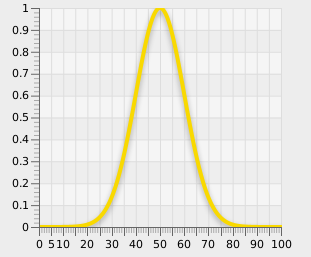
\includegraphics[scale=0.4]{membershipFunction}
		\caption{Funkce příslušnosti}
	\end{figure}


\end{frame}

\subsection{Fuzzy logika}
\begin{frame}{Fuzzy logika}
	
	\begin{itemize}
		\item AND reprezentován průnikem
		\item OR reprezentován sjednocením
		\item NOT reprezentován doplňkem
		\item definic IMPLIKACÍ je více
			\begin{itemize}
				\item např. Mamdani \(m_{a->b} = min(m_{A}(a),m_{B}(b))\)
			\end{itemize}
	\end{itemize}
	
	\begin{figure}[h]
		\centering
		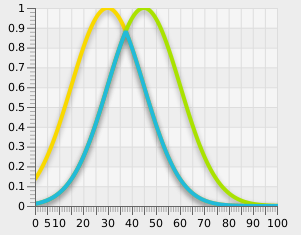
\includegraphics[scale=0.4]{fuzzyIntersection}
		\caption{Fuzzy průnik, AND}
	\end{figure}
	
\end{frame}

\subsection{Fuzzy inference}
\begin{frame}{Fuzzy inference}
	
	\begin{itemize}
		\item Modus ponens ve fuzzy logice
	\end{itemize}
	
	\begin{figure}[h]
		\centering
		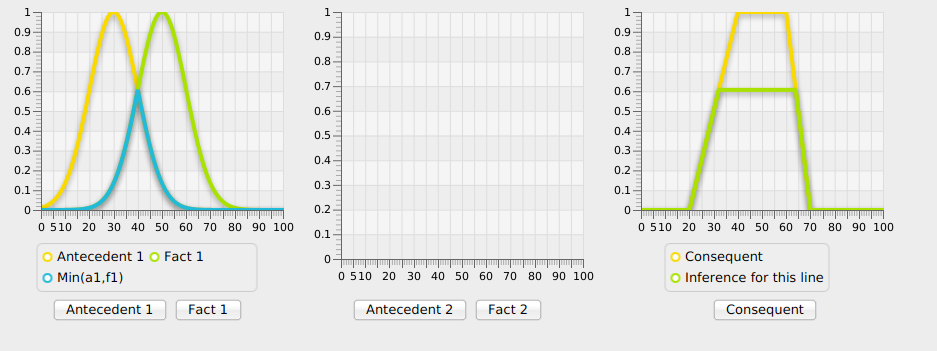
\includegraphics[scale=0.3]{oneRuleSimpleDetail}
		\caption{if A then B}
	\end{figure}
	
\end{frame}

\begin{frame}{Fuzzy inference}
	
	\begin{figure}[h]
		\centering
		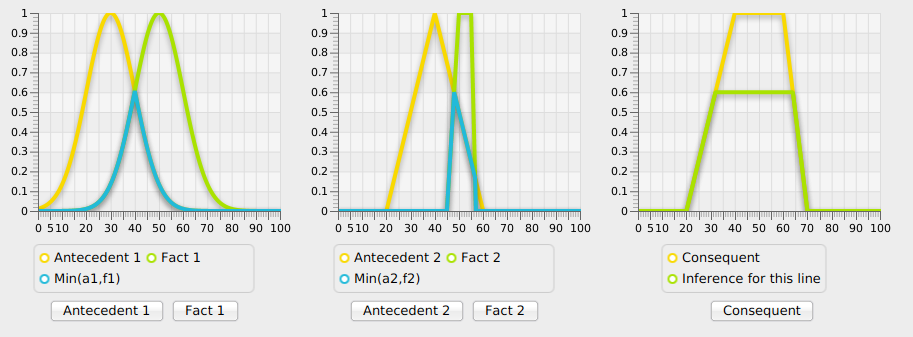
\includegraphics[scale=0.3]{oneRuleTwoFacts}
		\caption{if A and B then C}
	\end{figure}
	
\end{frame}

\begin{frame}{Fuzzy inference}
	
	\begin{figure}[h]
		\centering
		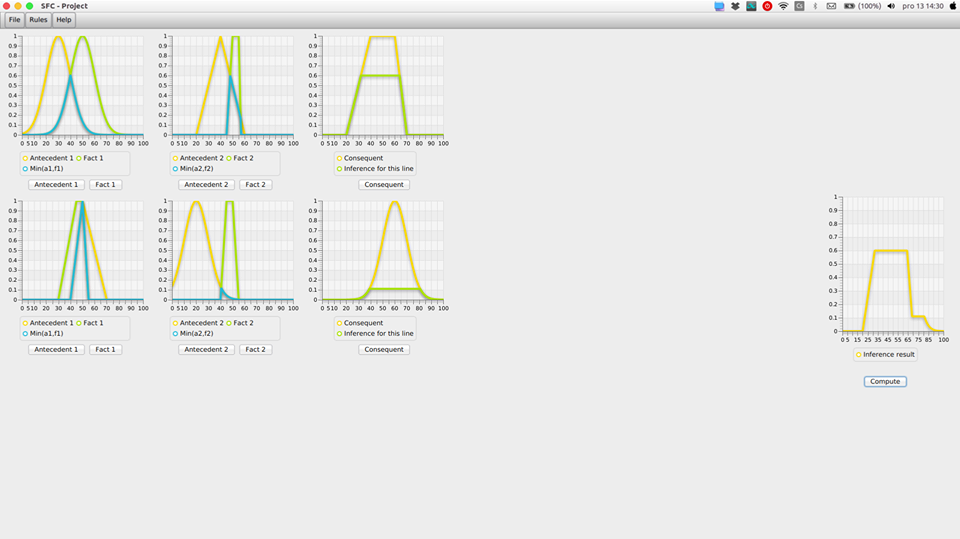
\includegraphics[scale=0.3]{twoRulesUpgraded}
		\caption{Dvě pravidla, dva předpoklady}
	\end{figure}
	
\end{frame}


\section{Závěr}
\begin{frame}[fragile]
\frametitle{Závěr}

\centering
Děkuji za pozornost.

\end{frame}

\end{document}
